\documentclass[11pt]{informatics-report}
\usepackage{color}
\usepackage[square,sort,comma,numbers]{natbib} 
\usepackage{comment}
\usepackage{url}
\usepackage{graphicx}
\usepackage{cleveref}
\usepackage{hyperref}
\graphicspath{ {Diagrams/}}
\usepackage{minted}


\title{6CCS3PRJ Final Year\\\vspace{0.2cm} LOST}
\author{Joshua Simpson}
\studentID{1225043}
\supervisor{Andrew Coles}

\date{\today}

\abstractFile{FrontMatter/abstract.tex}
\ackFile{FrontMatter/acknowledgements.tex} 

\begin{document}
\createFrontMatter
\onehalfspacing
\tableofcontents
\doublespacing


\chapter{Introduction}
Location based services have been developing rapidly over the past few decades, and are used in various aspects of technology - ranging from the route-planning software that is used to figure out a morning commute, to live time-tabling services that use bus or train positions to give accurate estimates on arrival times, to advertising based on the user's current location. It is safe to say that in some way or another, location services are prevalent in modern day life.

However, GPS\footnote{ Global Positioning System - a system using satellites to provide precise location information} -the most prominent form of location detection - only works to a certain level;  specifically to within a few feet at street level\cite{cook2005indoor}. Whilst achieving this level of precision a feat of engineering, it leaves a large market gap for providing truly localised contextually aware services. 

Contextually aware services are another rapidly developing technology, providing users with information or activities specific to their current location or situation, determining the suitability for such events by using sensor data\footnote{ Data such as location, temperature or time }. 

There are previous studies on using local area wireless access points to provide this sensor data at a level more precise than GPS can currently allow, but they are usually run in controlled environments, deriving a single mathematical equation in order to determine distance from the access point with high precision\cite{996891}. Unfortunately, this is impractical to apply as general use outside of a test environment.
\newline \newline 


\section{Project Aims}

The main goal of this project is to provide a proof-of-concept mobile application that can provide location and route-planning services whilst also delivering contextually aware services in a specific building - all without using GPS - demonstrating the possibilities that this area of application development holds for developers. Around this main feature, the project will aim to create software suite allowing for the efficent setup of a 'contextually aware building', as well as provide practical functionality to a variety of user groups ( by using the application to crowdsource data), to demonstrate the potential in this field. To achieve this, I will be collecting data on user location and wifi failure\footnote{A common occurence in the chosen building} throughout the building and providing a backend that displays this data in a useful manner.

To demonstrate a successful project, a large building with many potential locations is useful, as it shows the accuracy of of the location-finding and route-planning algorithms. To this end, the building that I am using to test this application is King's College London's Strand Campus\footnote{ It has not escaped my attention that this will also help all the new first years find Waterfront}. With roughly 17,000m2 of space and 9 floors to utilise, the application would not only be thoroughly tested but also most likely welcomed by King's 25,000 students\cite{headcount}.

\section{Report Structure}

This report will begin with a background on the project - taking a look at location based services and contextually aware services and the applications of both that are already available, along with an analysis of projects or papers that have attempted to solve the problem of location services at building level. This data will then be collated to analyse key problem areas during implementation. 

Following this there will be an outline of the requirements and specification for the project - showing both the project itself and the chosen extensions - complete with justifications on decisions made in the specification.


\chapter{Project Background and Main Points to Consider}

\section{Location Services}

Defined as \textit{"services that integrate a mobile device's location or position with other information so as to provide added value to a user"}\cite{schiller2004location}, the origins of location information services date back to 1973, when the US Department of Defence developed GPS to overcome the limitations imposed by navigation systems in use at the time\cite{national1995global}. This original system has since been developed into an integral part of many mobile applications, including mapping and route planning applications, as well as forming the 'sensor' in a lot of contextually aware applications. There is a well established method that is used in order to ascertain location, called trilateration\footnote{The process of finding a location by measuring distances, using geometry}. Triangulation\footnote{The process of finding a location by estimating the direction in which signals are coming from} is another method used to determine location, but is mostly inapplicable in the context of mobile devices\footnote{It is also commonly mistaken for trilateration}. Whilst I will not be developing an application that directly uses existing location technologies such as GPS, it is important to consider the practices used in such technologies when developing this project.

\subsection{Application: Google Maps}

Google Maps is easily the most widely used mapping tool on the planet, with over 54\% of smartphone owners using the app on a regular basis in 2013 ( for comparison, this was 10\% more than Facebook at the time)\cite{googlemaps}. Google Maps are a chief provider of location information services, with advanced route planning and street-view functionality. They serve this data through their own API\footnote{https://developers.google.com/maps/}. The most interesting aspect of their service ( in relation to this paper, at least ) is their recent addition of the use of Wireless Access Points for their location services. Whilst they do not rely solely on it for location, they do use the data to increase accuracy and speed through their Maps application\cite{googlewifi}. Interestingly, Google collect this WiFi data by crowdsourcing through an 'opt out' scheme in the Google Maps application\cite{googlewifi2} - this may not be possible in the case of this project ( as Google have used WiFi in a more assistive manner ), but it provides a good basis from which to approach the problem.

\subsection{Paper: Indoor Location Using Trilateration Characteristics}\cite{cook2005indoor}

This paper is especially relevant to the problem, considering the use of Wireless Local Area Networks in order to achieve trilateration. This is achieved by measuring the signal strength for at least 3 access points, and using the signal strength to determine the distance from the access point. Once you have three accurate distances you can essentially create a 'Venn Diagram' of where the user is located.

The paper goes on to state that there are inherent inaccuracies with this positioning technique, due to the variable nature of radio signals\cite{cook2005indoor}. 

To circumvent these inaccuracies, an elegant averaging method was developed, which started returning an accurate 'average signal strength' after 40 readings.

\subsubsection{Issues with the trilateration approach}
- As stated above, the trilateration approach has difficulties providing accuracies:

\textit{"Radio signals are extremely variable, particularly indoors, due to being reflected by obstacles or refracted round corners, known as multipath reflection. Environmental changes can also affect the signals, such as the number of people around. This means that the positioning technique is inherently inaccurate, with positions from raw Wi-Fi signals being in excess of 10m out. "}\cite{cook2005indoor}

\noindent- Whilst there is a solution designed to solve this problem in the case of the test environment, an application in a building such as Kings would require a number of different formulae in order to provide accurate signal strength averaging for different areas of King's\footnote{ Because of the variables such as distance between routers, building material, and the number of users in any area at a given time}

\noindent- Finally, in cases where the averaging solution is easily applicable, there \textit{should} be concerns regarding the impact on a mobile device's battery life when performing repeated scans and operations on the results of those scans.

\subsection{Paper: More Stuff on Location - Fuzzy Location?} 

\section{Context-Aware Services}

Contextually aware services are services that use data that pertains to the user or application's current situation to provide actions or functionality specific to that scenario. It is defined by Abowd as 

\textit{ "any information that can be used to characterize the situation of entities (i.e., whether a person, place or object) that are considered relevant to the interaction between a user and an application, including the user and the application themselves." }\cite{abowd1999towards}

Contextually aware services use 'sensors' to fetch this information - examples include location data, temperature, even the camera on your phone could be used as a sensor for contextual services\footnote{Consider how recent smartphones have software that stops the screen coming out of standby if it thinks it is in your pocket}.

\subsection{Estimote}

A rapidly accelerating tech start up, Estimote provides 'beacons' using low-power Bluetooth in order to send an ID\footnote{\url{http://estimote.com/api/getting-started/intro-to-beacons.html}} to an Estimote enabled application - these can then be programmatically associated with locations, events, etc. and calculates its distance from the phone using RSSI ( the received signal strength ) inside it's own API, meaning that it can be used very effectively to provide location-based services with minimal effort. This is so far the the most prominent product in the market using the iBeacon base.

Currently the major drawback of the Estimote is the price, which limits Estimote beacons / stickers to small buildings – covering an area such as King’s would be incredibly costly\footnote{\url{http://estimote.com/\#jump-to-products}}, and any structural changes regarding the beacons would require significant effort to represent in an application developed to use Estimote. Another issue is that - as stated above - using RSSI to fetch location information can become very complex in a large building with lots of people in it (which would cause signal attenuation at different levels throughout the day). 

\subsection{Google Maps}

As part of their vast toolset, Google Maps also has context-sensitive functions in it's API - an example is their 'Explore' feature\footnote{\url{http://google-latlong.blogspot.co.uk/2014/07/spend-more-time-exploring-with-google.html}}, which will show destinations of a certain type that are in the user's local area. The Explore function even takes into account time of day and weather in order to provide the best possible locations to the user.

An interesting point to note is that the 'Explore' function was predated by a 'Search Nearby' function that was removed\footnote{\url{http://www.jsonline.com/blogs/news/247119811.html}} - possibly due to privacy concerns\footnote{Covered later in Ethical Concerns}.


\subsection{Paper: An Architecture for Data Collection and Processing in Context-Aware Applications}\cite{salviarchitecture}

In this paper, Dario Salvi \textit{et al} pose that whilst Context Aware systems are showing and developing a greater use in general applications, that the field is not "applied in the real world"\cite{salviarchitecture}. The paper then goes on to propse an architecture that access and uses contextual data differently to provide the developer with more possibility to develop what is referred to as 'real world applications'.

Afterwards, the writers go on to set out three classes for collecting data - AtomicData\footnote{Singular pieces of information}, ContextData\footnote{Compositions of more than one piece of AtomicData}, and Relationships\footnote{Links between two ContextData}\cite{salviarchitecture}. These classes provide an interesting base for the data collection part of this project\footnote{ContextData holds the most interest, as I will need to collect multiple pieces of data}.

Overall the paper presents some very useful points on using contextual data to return usable information.

\section{Crowd Sourcing}

Crowd sourcing is generally defined as using a group of people or community to generate a needed resource. It is mostly thought of in terms of popular crowd-funding sites such as Kickstarter, or Indiegogo, but the term extends to other resources, such as data or ideas\footnote{For example, Cracked.com - a satire website - uses its own staff, but also looks for stories contributed by it's readers}. Generally, data crowdsourcing follows a pattern of clients paying for information that they need, and users that receive rewards to collect or generate this information.

\subsection{Captcha} 

Captcha was originally invented as an identification system to help discern humans from robots when performing tasks online. This started out as just a verification system ( which is growing more and more elaborate as robots evolve ), but was eventually evolved into an aid to digitizing books\footnote{\url{http://www.npr.org/2013/10/04/191620023/can-you-crowdsource-without-even-knowing-it}}. The most interesting point about this is that most of the users of Captcha have no idea that they are crowd-sourcing a huge effort every time they solve a Captcha.

\subsection{The 90-9-1 Rule for Participation Inequality in Social Media and Online Communities}\cite{participationinequality}

This article addresses a major problem with crowdsourcing data which Nielsen refers to as participation inequality, stating that user participation often follows a 90-9-1 rule, with 90\% of users being "lurkers or users that will observe but not contribute"\cite{participationinequality} . Nielsen also covers how to overcome this participation inequality (after briefly summarizing with ‘you can’t’); one method in particular is of interest when considering the aims of this project and its associated application: 'make participation a side effect'  – essentially the act of collecting data without the user having to do anything - this is less intrusive to the user’s day-to-day use of the application, but can also have obvious ethical ramifications if the user is unaware if they are sourcing data.

\section{Platform}

Because of the nature of the application being developed, it makes the most sense to develop for a mobile device - whilst devices like laptops offer more power to process information, the dataset that needs to be taken does not require the extra resources. Alongside this, mobile devices lend themselves better to the data-collection aspect of the project, with background services that can perform operations whilst the phone is inactive in a user's pocket. Finally, it is easier for a user to take out their phone in order to ascertain their location than it would be for a user to take out their laptop to perform the same operation.

With this in mind, the choice of platform then comes down to which type of mobile device to develop for - Android devices, or iOS devices. Whilst I could develop for both device types simultaneously using a platform such as Phonegap\footnote{http://phonegap.com/}, I have concerns about not using the native SDK for a platform - the abstraction provided by platforms such as Phonegap may reduce or restrict functionality that is necessary during development\footnote{Phonegap as an example, uses HTML, CSS and Javascript to create an application for both platforms simultaneously}. In the end, I decided to develop this for the Android platform alone.

\subsection{Reasons for Android as a platform}

The first point I considered whilst choosing a platform to use is the popularity of a platform - it makes sense to make the application available to the widest audience possible. In this case, Android dominates the market share, with 76.6\% of smartphones using the Android OS, compared to 19.7\% using iOS in the last quarter of 2014\cite{devicestats}.

Another major concern when deciding upon device was the functionality provided by SDKs for both Android and iOS. When I reviewed the functionality for both devices, I was unsurprised to find that iOS does not allow access to lower-level functionality. What did surprise me is that statistics like wireless signal strength was amongst these lower level functions\cite{ios1}\cite{ios2}\footnote{Whilst StackOverflow is not preferable as a citable source, finding an admission from Apple on this point is very difficult}. This restriction of access was a major concern\footnote{Unfortunately, later modifications to the application to circumvent issues with using signal strength meant this was no longer an issue}

\section{Ethical Concerns}

When developing an application that uses any form of personal information, there are definite privacy concerns. This is exascerbated when considering that there will be location information being returned to a server that is accessible by staff members. In this respect, it is important to not only adhere strictly to Data Protection laws, but also to consider the user's privacy and wellbeing. To this end, I need to make sure to collect the least amount of data I can, and to anonymise this data as much as possible in order to avoid sending any user details that would affect their privacy. Alongside this it would be prudent to secure the repository of any stored data against unauthorised users.

Another ethical point to consider is the code that is used to create this application. I should take due care to create this app using only my own code, except where express permission has been granted. In the same vein, I must make sure to adhere to all licenses for any libraries which I use in development.

\chapter{Requirements}
The client end of this project consists of two parts - an Android application that can determine user location ( LOST ) and provide route-planning inside the building, whilst feeding data to the backend, which will store the data and provide functions to view it as information. During implementation, I later developed a secondary Android application ( FOUND ) so that I could easily collect wireless data to test the application with. FOUND will not be available for users of the resulting software package for this project, however when considering possible extensions after the BSc report, FOUND would be an active component to allow for the easy mapping of a building in a bespoke software package. Because of the late addition of FOUND to the project, I will cover it briefly in Design, but give an in-depth analysis of the application in the Implementation section of this report.

\section{LOST - Android Application}

\subsection{Functional Requirements}
\begin{description}
\item[F1] - The application will be able to retrieve the most recent SQLite database containing wireless access point location information upon startup.
\item[F2] - The application will be able to accurately discern the user's location, using data provided by an SQLite database.
\item[F3] - The application will be able to provide the user with route-planning data, allowing the user to select a start and an end point, and provide the shortest path between the two points.
\item[F4] - The application will be able to discern whether the device is currently in the correct building for usage.
\item[F5] - The application will send anonymous information on the user's location to the backend periodically, if it is in the correct building
	\begin{description}
	\item[F5.1] - The user will be able to turn off this functionality
	\end{description}
\item[F6] - The application will periodically check if it has a functioning internet connection - if it is in the correct building. If the internet connection is malfunctioning, it will save this data.
	\begin{description}
	\item[F6.1] - Once the application regains internet access, it will send location data, and the MAC address of malfunctioning router to the backend.
	\item[F6.2] - The user will be able to turn off this functionality.
	\end{description}
\end{description}
\subsection{Non-functional Requirements}
\begin{description}
\item[NF1] - Application will not cause an 'ANR' ( app not responding ) error on any 'low-end' smartphone ( at time of writing, low end specifications are considered to be 1Ghz dual core processor and 768mb RAM\footnote{Figures created by comparing phone specifications at \url{http://www.phonearena.com/news/Affordable-not-cheap-15-best-low-cost-smartphones_id58696}}).
\item[NF2] - Application will provide location accurate to within 20 feet.
\item[NF3] - Application will use as little battery life as possible, using less than 5\% battery life within an hour.
\item[NF4] - Application will minimise data usage, making sure not to post data back using mobile data.
\item[NF5] - Application will not send data that can be used to identify the user, or any information that may be personal to the user / a breach of Data Protection laws.
\item[NF6] - Application will be usable on android versions 4.0.0 upwards, covering more than 90\% of android devices\cite{androidstats}.
\end{description}

\section{Backend}
\subsection{Functional Requirements}
\begin{description}
\item[F1] - Backend will operate a RESTful API that will allow the mobile application to post data to the server
\item[F2] - Backend will store POSTed data to an SQL database
\item[F3] - Backend will be retrieve data from SQL database, and display to user as information
\item[F4] - Backend will require user authentication to allow access to displayed data
\item[F5] - Backend will be able to store wifi location database, and serve it to a mobile device
\end{description}

\subsection{Non-functional Requirements}

\begin{description}
\item[NF1] - Backend will provide an easily navigable user interface
\item[NF2] - Backend will show data in an easily readable manner
\end{description}

\section{FOUND - Android Application}

\subsection{Functional Requirements}

\begin{description}
\item[F1] - Application will scan local wifi access points
\item[F2] - Application will insert the top access point into an SQLite database as a node, along with an edge connecting it to another node in the directed graph
\end{description}

\chapter{Design}
The application is split into two parts - therefore it will be detailed as a whole product, before the design of each component is analysed individually. Generally, the backend and the frontend application work as their own components, with the only interaction between the two being fetching the database, and sending data from the application to the database; because of this, an agile development cycle will be used. 

Further to this, a basic version of the Android application will be developed first, followed by an inital deployment of the backend, with the ability to receive data from the mobile application after that - from then, incremental additions will be made to either component, building for functionality first, then returning later for optimisation. 
\newpage

\section{Component Diagram}
\centerline{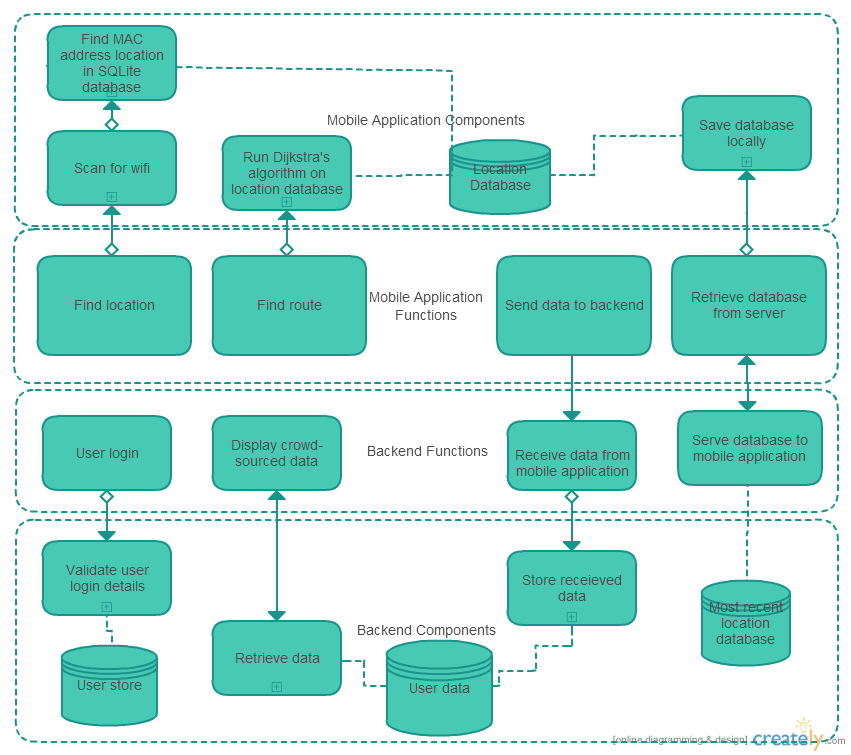
\includegraphics[scale=0.6]{ComponentDiagram}}
\newpage

\section{LOST}

The 'front end' of the project, the LOST application provides most of the functionality detailed in the earlier chapters of this report. In this section, I will go into more detail as to what each function will need to do in order to provide the outlined functionality. You will find a \nameref{UseCase}, along with wireframes for each aspect in the Appendix. For clarification, each 'view' in an Android Application is called an Activity.

\subsection{Finding Location}

This is one of the most critical aspects of the application, and also one of the most challenging as a great deal of consideration needs to be paid towards efficiency, accuracy, and precision - it will generally be more expensive in terms of resources, and in fact battery power, to increase the precision.

In order to ascertain location, the application will need to perform a scan of nearby wireless access points. The MAC address and signal strength of each access point will be collected, and put in descending\footnote{Or considering how signal strengths are measure, ascending. Signal strength is measured in DBm and measure as negative figures. The 'quieter' a signal is, the weaker it is - therefore a signal strength of -10 is much more powerful than a signal strength of -80} order of strength.
The original intention\footnote{Results of this will be detailed in the 'Implementation' section of this report.} at this point was to use actual signal strength figures to get the most precise location information, as done by Cook \textit{et al}\cite{cook2005indoor}. 

To get this location information, the top three MAC addresses in the list would be used to filter the location database down to a single node, representing that location\footnote{Discussed further in the Databases section}. This location would then be displayed to the user, along with an option to refresh this ( performing another scan, incase the user doesn't think they are in the right location ). There will also be a button that allows the user to use their given location as the start or end point for route planning.

\subsection{Route Planning}

This function ties in with the location finding function of the application - the user will either be able to load it normally, or load it from the 'Location Finder' part of the application - if this is the case then either the 'to' or 'from' sections of the application will contain the user's location.

Regardless of how the activity is accessed, there will be two drop down lists, allowing the user to select the start and end points. The application will translate these selections into nodes in the directed graph created from the location database, and perform Dijkstra's algorithm to find the shortest path between the two locations. The nodes traversed in this path are displayed in order on the next Activity to show the user the path they need to take as a step-by-step route. A possible extension on this once functionality has been implemented would be to have each step highlight green when the user reaches the associated location, however this would most likely be done through repetitive wireless scanning, so steps would need to be taken to ensure that this doesn't rapidly drain battery. 

\subsubsection{Choosing an algorithm}

Because of the limited power available to a mobile device, alongside the short attention span of users\footnote{And indeed Google's limit before declaring an application unresponsive}, it was important to select the most efficient algorithm for the problem being faced. Another algorithm which could have been used in this instance would have been Bellman-Ford's algorithm. After research into, and a comparison of, the two algorithms it is shown that Dijkstra's algorithm is much more efficient than Bellman-Ford's\cite{thippeswamystudy}, with the latter being used only in the case of directed graphs with negative edge weights ( a situation that Dijkstra's algorithm is not equipped to deal with ) - as there are no negative edge weights when travelling from one area to another, Dijkstra's algorithm is clearly the best choice.

\subsection{Recognising access point faults}

One of the chosen forms of data to upload is faults with access points, as this shows a useful application of the concepts that form the foundation of this project. In order to retrieve this data, the mobile application needs to be able to recognise when it is in Kings, when it is using a Kings wireless access point, and when that access point is having issue. However, there is an obvious issue when trying to upload data about malfunctioning access points - the lack of internet. To solve this, we need to add functionality for caching data.

\subsubsection{Caching Data}

Because there will be times when collected data can not be sent back to the server ( either through malfunction or lack of connection ), it is important to keep the data - making sure it is properly timestamped for when it is uploaded - and then upload it when a connection becomes available again. An important problem to consider here is that data may become irrelevant if it is uploaded after too long a period of time, so it is worth looking into functions that clear items of a certain age out of the cache. 

\subsection{Data Upload}

This function will run at regular intervals in the background, regardless of whether the app is open, as the chances of the user having the app open all the time are very slim - studies show that an average app sessions lasts barely more than a minute\cite{Bohmer:2011:FAA:2037373.2037383}. Because this will be a repeating task running in the background at any time, it is imperative that the task is threaded properly, so as to avoid blocking the main thread with what could potentially be a long task. 

Also important is to consider how regularly the information is sent - if the information is sent too frequently it will be a needless waste of resources, and will leave the resulting data set far larger than it needs to be, but too little and the resulting data set will be insubstantial. It was decided that an interval of 15 minutes is appropriate, as it is frequent enough that people may have moved areas, but infrequent enough that it won't use too many resources.

\section{Backend}

The backend of the project, the web server will receive and present crowd-sourced data to authorised individuals. As a secondary function, it will also serve the locations database up to the mobile application - allowing for the storage and retrieval of the latest version incase the architecture of the building changes; either physically ( which is unlikely ), or logically ( where wireless access points are added, changed, or removed ). A critical aspect, in order to maintain trust, and compliance with Data Protection laws, along with the BCS Code of Conduct, is to limit the access to the data to only those who need it.


\subsection{Public API - Receiving data, and serving the location database}

The backend will need to present a RESTful API, that the mobile application can POST data to. Once data has been POST'ed to these API endpoints, the server will need to validate the data before finally storing it. It is important that the API isn't subject to blocking - whilst efforts will be made to stagger uploads from the user end \footnote{Spreading operations instead of having the server deal with all of them at once}, it is important to make sure that the server deals with them all in a timely manner, and can handle lots of operations simultaneously.

Another function of the API will be to receive requests for the locations database, and serve that database to the mobile application - usually for the first startup of the application, but also if any data in the database changes.  

\subsection{Data Presentation}

The server also needs to be able to retrieve the data it has stored and present it to an authorised user in a way that converts it from \textit{data} into \textit{information} - this means presenting it in a manner that is easy to read, and provides some function to the user. Originally, it should be able to just display the data to the user in a list ( where an access point has a fault / when people are in a location ) - but this should be expanded on, providing an analysis of the data and providing it in different forms, such as charts showing the usage of an area over a particular amount of time. An important extension to this would be to provide the user with a way to export the dataset out, so that they can generate information suited to their own needs.

\subsection{Security}

It is important that all the data on the server is only accessible by authorised users - this means that a login should be required to access the site provided by the backend, along with any databases / data sources that it utilises. Further to this, any data that is sent in should be completely anonymised - whilst this is mostly a function of the mobile application, it would be pertinent to maintain this vigilance in all areas of the project. An example of how to anonymise the data at the backend would be to make sure that no data regarding the origin of the data is stored beyond that which is expected. If the aforementioned data does need to be stored, then the same standard of security applied to the rest of the backend should also be applied to this data.


\section{Databases}

At the end of this product, there will only be two databases in use - the locations database served by the backend and used by the mobile application, and the database that will store the data uploaded by the mobile application. The structure of these databases needs to be clearly defined as early as possible, so as to avoid having to make structural changes during development. 

\subsection{Locations Database}

The locations database will comprise of two tables - Nodes, and Edges, and will allow for the building of a directed graph in-application that can be used to find the shortest path to a location.

\subsubsection{Nodes}

The nodes table will contain nodes that represent each location that has been mapped in Kings. Its fields will be: 

\begin{description}
\item[ID] - ID of node, stored as an integer
\item[Name] - Name of location, stored as a string
\item[MAC] - MAC address of the corresponding wireless access point\footnote{Originally three MAC addresses for precision, but reduced to one after encountering issues as mentioned in 'Implementation'} - stored as a string
\end{description}

\subsubsection{Edges}

The edges table will contain edges that represent connections between nodes. Its fields will be:

\begin{description}
\item[ID] - ID of edge, stored as an integer
\item[StartNode] - The ID of the node that the edge begins at, stored as an integer
\item[EndNode] - The ID of the node that the edge ends at, stored as an integer
\item[Weight] - The amount of time taken to get from the StartNode to the EndNode, stored as an integer.
\item[Method] - Not definite, as could be implied by the weight, but the method used to get from one node to another ( either walking or taking the lift in the case of KCL ). Stored as a string. 
\end{description}

\subsection{User Data}

This database will contain the data that has been uploaded as people have used the mobile app - the data contained in this database will vary from table to table, depending on the sort of data that we want to collect from the user. Because of this, we will define a couple of example databases, as the other possibilities for collected data are endless. 

\subsubsection{Location Reporting}

An example database showing the locations / facilities in Kings that are being used in Kings, demonstrating the usability of both crowd-sourcing data and contextually aware mobile applications. 

\begin{description}
\item[ID] - ID of information upload, mostly for indexing purposes. Stored as an integer.
\item[Location] - A string showing where the user was when the data was uploaded. Stored as a string.
\item[Time] - Date / Time that data is recorded ( which may well be different from the time of upload ), stored as a string.
\end{description}
\newpage

\subsubsection{Access Point Recording}
\begin{description}
\item[ID] - ID of information upload, mostly for indexing purposes. Stored as an integer.
\item[MAC] - MAC address of reported access point. Stored as a string.
\item[Location] - Location of issue. Stored as a string.
\item[Time] - Date / Time that data is recorded. Stored as a string.
\item[Notes] - Notes about the issue - to be used by users of the backend. Stored as a string.
\item[Time uploaded] - The time that the data was pushed to the server. Stored as a string.
\end{description}

\chapter{Implementation}

In this section I will cover the implementation of the various parts of the project in greater detail, explaining the various components that make up these parts, and the choices behind them.

\section{LOST}

\subsection{Toolkit}

\subsubsection{Languages Used}
As an Android application, LOST was written almost completely in Java, using XML for layout files and SQL to manage the database. Whilst there is the option to use C / C++ to write directly for the Linux operating system that Android is based on, it is not recommended by Google.

\subsubsection{Development Environment}

When I started developing LOST, I was using Eclipse - however about a month in I switched from Eclipse to IntelliJ for several reasons. Eclipse seemed to be inherently bug-ridden, requiring a restart frequently which was disruptive to work-flow. Alongside this, IntelliJ made much better use of available plugins - including plugins that provided great Git integration, which I used for version control. 

Whilst developing, each build was tested on two Android phones - one older, now low-end phone, and one much more recent high end phone, providing a good analysis of application performance over different devices.

\subsubsection{Libraries / Frameworks Used}

Whilst developing LOST, I used three different libraries - two of which were critical to the implementation of the application, and a third which provided ease of use whilst developing. 

The first library used was the Google Play App Compatibility support library\cite{appcompat} - this library allows developers to use Android components on older devices that have been introduced in newer implementations of the Android operating system, providing greater coverage and compatibility. 

The second library I used was the Apache Commons library, which provided functionality to perform the network operations necessary to upload data to the server - most importantly it allowed for the crafting and delivery of HTTP POST requests.

The third library was the SQLiteAssetHelper library, which provided an extension to the SQLite functionality already included in the Android API. It searches for database files in all the directories that assets would normally be put in, and allowed easy manipulation of databases across different devices.

\subsection{Component Analysis}

In this section I will provide an analysis of each class in the application, along with the functions that are performed within each activity.

\subsubsection{Activity: Main Menu}

The first activity a user will see upon opening the application - at first glance this activity just stands as a gateway to the rest of the application, but as soon as the application has started up, it retrieves the latest version of the locations database, and then opens that database to build a directed graph, using the DiGraph class. Finally, it kickstarts the background service that pushes data to the backend.

It was important to make sure that this operation in the background ran in a seperate thread to the GUI, or there would have been issues with blocking whilst the operation was carried out ( problems that would become more prevalent the larger the database became ).

\subsubsection{Class: DiGraph} 

This class is critical to the function of the application - with all of the location based functions in the application using stored in an object of this class. The DiGraph class uses custom made Node and Edge classes to create a directed graph within the application, allowing for the later implementation of Dijkstra's algorithm. Each Node represents a location within Kings, with each Edge representing a connection between those two locations.

One of the most critical aspects of the class is the global variable that forms its adjacency list, details each Node's adjacent Nodes, and the Edges that connect them. Finding a data structure in which to store these three pieces of information, whilst also making them easily retrievable was difficult - eventually a HashMap within a HashMap was used. 

In order to allow for the easy retrieval of nodes using different identifying factors, it was necessary to implement a rough type of custom indexing, which involved taking the Nodes that were in the adjacency list and creating Maps for them for any data type that would be needed to call a Node. An example would be:

\begin{minted}[frame=single]{Java}
public static Map<Integer, Node> nodeIDList;
public static Map<String, Node> nodeLocationList;
public static Map<String, Node> nodeMAC;  
\end{minted}

Each map in the above code stores a seperate copy of the list of Nodes, with whichever data is used to find it using the .get() method. For example, using 

\begin{minted}[frame=single]{Java}
nodeIDList.get(0);
\end{minted}
would be the same as

\begin{minted}[frame=single]{Java}
nodeMAC.get("MAC address of the first Node");
\end{minted}

The problem with this approach is that when originally adding each Node to the DiGraph, the operation is now much more expensive to perform, and there is exponentially more space used per Node - however the ability to easily retrieve each node offsets this initally expensive operation, and the memory usage is still negligible in terms of the memory available to the device.

\subsubsection{Activity: Location Finder}

When this activity is opened, a wifi scan is immediately performed, and a loading screen shown until the Activity has received and processed the results. The completion of a wifi scan triggers a WIFI\_SCAN\_RESULTS\_AVAILABLE event which is listened for by the BroadcastReceiver class. When the BroadcastReceiver receives this action, it triggers an onReceive method where the results can be fetched and operations run as a response to this action.

The results are returned in a <ScanResults> List, which is then ordered using a comparator, according to signal strength ( from the best quality to the lowest quality ). The top result is taken, and its MAC address used to find the Node relevant to that user's location in the DiGraph. Finally, the user's location is extrapolated by getting the 'location' variable from the Node.

The original plan for this class involved using the top three access points to get a much more precise estimate of the user's location using trilateration. Unfortunately, because of the variation of signal strengths at any given point ( a figure that can even be affected by another person's body ), the top three MAC addresses in any given place can change constantly. To get an accurate result would require having populated the database with every possible variation for every area, resulting in an exponential increase in the amount of data that needs to be taken ( and therefore Nodes required ). 

Once this activity has pinpointed your location, the loading screen will be replaced by that location, along with a button to refresh the location ( which will start another scan ), and a button that will use the current location as the start point in the route planning activity.

An interesting feature provided by the BroadcastReceiver is that it will listen for \textit{any} trigger of the SCAN\_RESULTS\_AVAILABLE action, meaning that when the system performs a wifi scan seperate from the application, the application will perform the operation defined in it's onReceive anyway - this means that the location will auto-update without having to trigger multiple scans, ultimately meaning a more economical use of resources.

\subsubsection{Activity: Route Planning}

This activity provides two drop down lists - each populated with all of the locations that are currently present in the directed graph. The user can select a start point, and an end point and once the 'Find Route' button has been pressed, the activity fetches the relevant nodes for both locations ( by using their position in the drop down lists as the node ID, and fetching from the nodeIDList ). It then applies Dijkstra's algorithm to the start node to find the shortest distance to all of the nodes in the directed graph, before using the second node as an argument to find a path between the two.

The resulting path is then displayed in the next activity - each step in the path is used to create an 'inflatable' - inflatables allow for the dynamic creation of activities by using the same small section of the layout and filling it with changeable content.

\subsubsection{Class: Dijkstra}

Dijkstra's algorithm is the chosen shortest path algorithm for this project, and provides all of the functionality behind the route planning activity. The implementation of Dijkstra's algorithm written for this project will take a directed graph object upon instantiation of a 'Dijkstra' object:

\begin{minted}[frame=single]{Java}
DiGraph dg = MainActivity.myGraph;
Dijkstra pathFinder = new Dijkstra(MainActivity.myGraph);
\end{minted}

To run the algorithm, it is passed a source node:

\begin{minted}[frame=single]{Java}
pathFinder.execute(dg.getNodeFromID(start.getSelectedItemPosition() + 1));
\end{minted}

This finds the shortest path for all nodes from that source node, filling out the 'predecessors' map variable with pairs containing the node, then the node preceding it. To retrieve a path, a LinkedList is generated by stepping backwards from a given end node:

\begin{minted}[frame=single]{Java}
LinkedList<Node> pathList = pathFinder.getPath(dg.getNodeFromID
	(end.getSelectedItemPosition() + 1));
\end{minted}

\begin{minted}[frame=single]{Java}
public LinkedList<Node> getPath(Node target) {
        LinkedList<Node> path = new LinkedList<Node>();
        Node step = target;
        // Check if a path exists
        if (predecessors.get(step) == null) {
            return path;
        }
        path.add(step);
        while (predecessors.get(step) != null) {
            step = predecessors.get(step);
            path.add(step);
        }
        // Put it into the correct order
        Collections.reverse(path);
        return path;
    }
\end{minted}

\subsubsection{Service: LocationPush}

Services are components within Android applications that can perform operations in the background that don't require a graphical user interface\cite{androidservices} - therefore it serves as the perfect platform from which to routinely push data without requiring user input.

Firstly, it is worth noting that a Service does run in the main thread of it's hosting process - therefore any long running operations should be be run within a new thread so as to avoid blocking on the main.

The first thing the service does is trigger a wifiscan in much the same manner as the Location Finder activity does - the main difference being that when the BroadcastReceiver is triggered the first time, it is then unregistered to prevent the repeated triggering of the operation defined in it's onReceive.

After this first trigger, the Service will create a new thread, and attempt to connect to google - if it cannot connect it will check the status of the internet connection and then create a 'fault' record in an SQLite database, noting the time and any details that can be provided as to where the failure occurred. If it can connect, the Service will POST the location data in JSON format, before checking to see if there are any faults in the aforementioned database - if there are it will POST each fault individually in JSON format\footnote{Expensive, no?}.

Finally, the thread will sleep for 15 minutes - upon waking, it will register the BroadcastReceiver again so that it can listen for the next SCAN\_RESULTS\_AVAILABLE action that the device provides. This again allows for an economical use of resources whilst running in the background, instead of triggering a wifiscan itself every 15 minutes:


\begin{minted}[frame=single]{Java}
public void onReceive(Context c, Intent intent) {
            unregisterReceiver(this);
            new Thread(new Runnable() {
            	....
SystemClock.sleep(900000);
registerReceiver(scanReceiver, 
	new IntentFilter(WifiManager.SCAN_RESULTS_AVAILABLE_ACTION));
}.start();

\end{minted}

\subsubsection{Activity: Settings}

This Activity provides very little towards functionality, instead providing utility. Firstly, it provides a warning to the user that the app will collect data at regular intervals, and provides checkboxes that allow the user to opt out of the data collection. During development, another feature was also added to provide more utility to the user - a button that will open a dialog for the user to enter their King's username and password.

This data is then used to create correctly set up wireless profiles for both AccessKings and Eduroam. This idea is meant to provide more functionality to the user from the application, and also helps to make sure that the user doesn't have connection issues due to authentication when in Kings.

Unfortunately, during implementation there was a major issue discovered - the functionality to programatically add a wireless profile for a WPA-Enterprise network was only added in 4.3, and so far is not available for earlier Android versions. An implementation using this would violate non-functional requirement NF6, so if this application were to progress beyond the BSc report, multiple versions of the application would be supported using Google's multiple APK support.

\subsection{Difficulties during implementation}

Whilst developing the mobile application I encountered the majority of the difficulties for this project - mostly due to having to implement complex methods such as a functioning Dijkstra's algorithm, but mostly trying to develop a method to determine the user's location that was accurate, with as much precision as possible. After extensive testing, it became clear that the originally planned '3 MAC' method, where I would use a combination of trilateration and fuzzy location determination\footnote{A method for roughly determining location} to determine a precise\footnote{To within 5-10 feet} location, however the rate of success for accurately finding the user's location was too low - most of the time the application returning that it didn't recognise the area - this is mostly due to the original implementation.

This original implementation took the top three MAC address and concatenated them, meaning that to find a match the user had to be in the location where that exact combination happens again - however, as covered by Cook et al, radio signals are extremely variable\cite{cook2005indoor}, and this had a major impact. 

Because of the limited amount of time available, it was necessary to establish a working, accurate proof-of-concept before trying to develop a higher level of precision, and so the current implementation is almost guaranteed to find your location within Kings\footnote{ 'Almost' because of mobile wireless hotspots and the like causing inaccuracies }. 

\section{Backend}

\subsection{Toolkit}

\subsubsection{Languages Used}

To develop the backend I looked into the functionality provided by a few different languages - with very little grounding in web server development it was important to pick a language that wouldn't turn out to lack functionality that I required later on.

Eventually, Ruby was chosen as the language, using the Ruby on Rails web framework to develop the backend. Ruby on Rails allows for rapid prototyping, so I could focus on implementing functionality quickly and effectively. As a proof-of-concept project, this was an important factor in choice\footnote{Admittedly another was that Ruby on Rails is 'optimised for programmer happiness'}.

\subsubsection{Development Environment}

Setting up an optimal development environment for the backend was much tricker than for the Android application, but there were several tools that streamlined the process. Firstly, a Digital Ocean server was rented for the duration of the project - Digital Ocean provide 'ready to deploy' droplets - essentially allowing me to rent a server that came with a version of Ubuntu and any web server stack already installed - after this I just had to familiarise myself with the server and the language itself.

Outside of this server, I used Sublime text editor, along with the SFTP plugin to edit files locally and push them back to the server - this was mostly when I was implementing larger functions - for smaller functions I would use SSH and Vim. Also useful was the Rails console, which provided a shell to test code in before implementing it in the application proper.

\subsubsection{Libraries / Frameworks Used}

Libraries in Rails are given the name 'Gems' - implementing them in a Ruby on Rails ( RoR ) server is fairly easy to perform and they can provide some great additional functionality that would be difficult / time-consuming to write from scratch. To this end I used two Gems that aren't automatically packed with RoR.

Devise was the first Gem - Devise provides easily implementable user and session management, allowing for the quick development and continued rapid prototyping of a strong authentication system. To write my own user authenticaton with a Gem like Devise available would have been a waste of time, and almost definitely would not have provided the completeness of security that Devise does. 

The other Gem that I used was the Bootstrap Gem. Bootstrap, developed by Twitter, provides a front-end framework for easy deployment of intuitive, good looking sites. It also focuses on making any front end-code written responsive - meaning that it will run effectively on mobile phones. Whilst this wasn't critical, the overall package allowed for rapid-prototyping much easier by alleviating any concerns as to the front-end. As a developer that works mostly with back-end / functional code, this was a highly valuable Gem.

I also used one Javascript API called Highcharts - Highcharts provides an API for charting data, allowing the development of good looking data visualisation views. This was crucial for turning the stored data into information, and whilst it took some work to get Highcharts working well with RoR, it was time well spent and Highcharts helped to develop professional looking charts that would not have been possible had I wrote the function myself.

\subsection{Component Analysis: API}

In this section I will run through each endpoint of the API, showing the data the JSON that it takes in, and the action performed when each endpoint is consumed.

\subsubsection{POST: /locations}

When a JSON of the form :

\begin{minted}[frame=single]{JSON}
{"loc" : location, "time" : time-of-record}
\end{minted}

is POSTed to the above endpoint, the server will create a new location record, with the value of 'location' as it's location, and using 'time' as the time recorded. This is one of the most used endpoints, as it is the endpoint that the mobile application posts to every 15 minutes.

\subsubsection{POST: /accesspoints}

When a JSON of the form :

\begin{minted}[frame=single]{JSON}
{ "mac" : mac, "location" : location, "time" : time, "notes" : notes }

is POSTed to the above endpoint, the server will create a new access point fault record, using each of the key-value pairs in the JSON post for the relevant field in the database.

\subsubsection{POST: /dbs}

This endpoint is reserved for the secondary mobile application, designed to allow for the easy sharing of a locations database created within the application. When a file is posted to this address, it is stored on the server, under the path /public/dbs/.

\subsubsection{GET: /dbs/get}

This endpoint allows the main android application to fetch a created locations database from the server - a GET request will return the database file.

\subsection{Component Analysis: Site}

The frontend of the server presents the data that has been collected through the mobile application to an authorised user - firstly as raw data, but with the option to view the data in graph format. 

\subsubsection{Index}

The root of the site provides a fragment view of the data that a user could see by clicking on the relevant section of the site - it displays a small portion of the current Access Point Fault list, along with a chart showing total location usage over the past 7 days.

\subsubsection{Locations}

The locations list shows each record that has been created by a POST from the mobile application, with the details of which location the record was created at, and the timestamp for the record. There are links on each row to either view or delete the record. When the record is viewed, the user is taken to a page showing the usage of that location over the past 7, 14 and 28 days. 

Additionally, from the main locations list, the user can click a button at the bottom which will download the entire list in .csv format, allowing the user to load the dataset into their own program and create their own information sets from there.

\subsubsection{Access Point Faults}

The access point faults list functions in much the same way as the locations list, showing the MAC address of the malfunctioning access point, along with it's location, the timestamp for when the problem was discovered, and any notes pertaining to the issue. The options for each of these records are either 'Show', 'Delete', or 'Edit'. Show will take the user to a page that shows only that record's details. Delete will delete the record, and Edit allows the user to modify the record - allowing for the updating of the Notes field. 


%\chapter{Report Body}
The central part of the report usually consists of three or four chapters detailing the technical work undertaken during the project. {\bf{\textcolor{red}{The structure of these chapters is highly project dependent}}}. They can reflect the chronological development of the project, e.g. design, implementation, experimentation, optimisation, evaluation, etc (although this is not always the best approach). However you choose to structure this part of the report, you should make it clear how you arrived at your chosen approach in preference to other alternatives. In terms of the software that you produce, you should describe and justify the design of your programs at some high level, e.g. using OMT, Z, VDL, etc., and you should document any interesting problems with, or features of, your implementation. Integration and testing are also important to discuss in some cases. You may include fragments of your source code in the main body of the report to illustrate points; the full source code is included in an appendix to your written report.

\section{Section Heading}

\subsection{Subsection Heading}
%\chapter{Design \& Specification}

\section{Section Heading}
%\chapter{Implementation}

\section{Section Heading}

%\chapter{Professional and Ethical Issues}
Either in a seperate section or throughout the report demonstrate that you are aware of the \textbf{Code of Conduct \& Code of Good Practice} issued by the British Computer Society and have applied their principles, where appropriate, as you carried out your project.

\section{Section Heading}

%\chapter{Results/Evaluation}

\section{Software Testing}

\section{Section Heading}

%\chapter{Conclusion and Future Work}

The project's conclusions should list the key things that have been learnt as a consequence of engaging in your project work. For example, ``The use of overloading in C++ provides a very elegant mechanism for transparent parallelisation of sequential programs'', or ``The overheads of linear-time n-body algorithms makes them computationally less efficient than $O(n \log n)$ algorithms for systems with less than 100000 particles''. Avoid tedious personal reflections like ``I learned a lot about C++ programming...'', or ``Simulating colliding galaxies can be real fun...''. It is common to finish the report by listing ways in which the project can be taken further. This might, for example, be a plan for turning a piece of software or hardware into a marketable product, or a set of ideas for possibly turning your project into an MPhil or PhD.


\bibliographystyle{plain}
\bibliography{mybib}
\addcontentsline{toc}{section}{Bibliography}
\appendix
\include{Appendices/appendix}
%\chapter{User Guide}
\section{Instructions}
You must provide an adequate user guide for your software. The guide should provide easily understood instructions on how to use your software. A particularly useful approach is to treat the user guide as a walk-through of a typical session, or set of sessions, which collectively display all of the features of your package. Technical details of how the package works are rarely required. Keep the guide concise and simple. The extensive use of diagrams, illustrating the package in action, can often be particularly helpful. The user guide is sometimes included as a chapter in the main body of the report, but is often better included in an appendix to the main report.

%\chapter{Source Code}
\section{Instructions}
Complete source code listings must be submitted as an appendix to the report. The project source codes are usually spread out over several files/units. You should try to help the reader to navigate through your source code by providing a ``table of contents'' (titles of these files/units and one line descriptions). The first page of the program listings folder must contain the following statement certifying the work as your own: ``I verify that I am the sole author of the programs contained in this folder, except where explicitly stated to the contrary''. Your (typed) signature and the date should follow this statement.

All work on programs must stop once the code is submitted. You are required to keep safely several copies of this version of the program - one copy must be kept on the departmental disk space - and you must use one of these copies in the project examination. Your examiners may ask to see the last-modified dates of your program files, and may ask you to demonstrate that the program files you use in the project examination are identical to the program files you had stored on the departmental disk space before you submitted the project. Any attempt to demonstrate code that is not included in your submitted source listings is an attempt to cheat; any such attempt will be reported to the KCL Misconduct Committee.

\textbf{You may find it easier to firstly generate a PDF of your source code using a text editor and then merge it to the end of your report. There are many free tools available that allow you to merge PDF files.}


\end{document}
